\chapter{Continuity}
In this section we will cover the topics related to the continuity of functions from one topological space to another topological space. Also, we will put much emphasis on the properties of continouse functions from one metric space to anther metric space (in particular functions from $\R \to \R$). The notion of continuity is one of the central concepts in analysis which shows up anywhere there is a trace of analysis!

\section{Basic Definitions and Characterizations}
We start with the most general definition of a continouse function in a topological setting.

\begin{definition}
	Let $(X,\mathcal{T}_X)$ and $(Y,\mathcal{T}_Y)$ be two topological spaces. We say a function $f: X \to Y$ is continouse [on $(X,\mathcal{T}_X$] iff
	\[ \forall G \in \mathcal{T}_Y \wh \inv{f}(G) \in \mathcal{T}_X. \]f
	Note that $\inv{f}(G)$ means the pre-image of the set $G$, and does not mean the inverse of the function $f$.
\end{definition}
In words, a function from $X$ to $Y$ is continouse if the pre-image of every open set in $Y$ is also an open set in $X$. 

\begin{lemma}
	$f: X \to Y$ is continouse if and only if $\inv{f}(C)$ is closed for every closed set $C$ in $Y$.
\end{lemma}

\begin{proof}
	First, we need to prove the following identity
	\[ \inv{f}(C^c) = (\inv{f}(C))^c. \]
	To show this we first show $\inv{f}(C^c) \subseteq (\inv{f}(C))^c$. Let $x \in \inv{f}(C^c)$. Then
	\begin{align*}
		x \in \inv{f}(C^c) \implies f(x) \in C^c \implies f(x) \notin C \implies x \notin \inv{f}(C) \implies x \in (\inv{f}(C))^c.
	\end{align*}
	Then we need to show $ (\inv{f}(C))^c \subseteq \inv{f}(C^c) $. Let $x\in(\inv{f}(C))^c$. Then 
	\[ x\in(\inv{f}(C))^c \implies x \notin \inv{f}(C) \implies f(x)\notin C \implies f(x) \in C^c \implies x \in \inv{f}(C^c). \]
	Thus we proved that $\inv{f}(C^c) = (\inv{f}(C))^c$. Now to prove the lemma, for the $\implies$ direction, we assume that $f$ is continouse. Let $C \subseteq Y$ be a closed set. Then $C^c \in \mathcal{T}_Y$. Since $f$ is continouse, then $\inv{f}(C^c) \in \mathcal{T}_X$. From the identity we proved above, it immediately follows that $(\inv{f}(C))^c \in T_x$, thus $\inv{f}(C)$ is closed.  Now for the other direction, we assume that $\inv{f}(C)$ is closed for every closed set $C$ in $Y$. Let $G \in \mathcal{T}_Y$. Then $G^c$ is closed. From our assumption, we know that $\inv{f}(G^c) = (\inv{f}(G))^c$ is closed. Thus $\inv{f}(G) \in \mathcal{T}_X$. So the pre-image of $G$ is open. Then we conclude that $f$ is continouse.
\end{proof}

\begin{example}
	In any metric space $(X,d)$, for any point $p \in X$, the function $f: X \to \R$ defined as
	\[ f(x) = d(x,p), \qquad x\in \R, \]
	is continouse. \\
	\begin{proof}
		To show this, we need to show that $\inv{f}(G)$, where $G$ is open in $\R$, is open in $X$. Let $U = (a,b)$ be an interval in $\R$ for some $a,b\in\R$. We will have three cases of such interval, where $a>0,b>0$, $a<0, b>0$, and $a<0, b<0$. In the third case, $\inv{f}(U) = \emptyset$ which is indeed open. For the first case, we have
		\[ \inv{f}(U) = \ballCO{p}{b} \backslash \ballCC{p}{a} = \ballCO{p}{b} \cup (\ballCC{p}{a})^c. \]
		The right hand side is the intersection of two open sets. Thus $\inv{f}(U)$ is open. For the second case, where $a<0, b>0$, the calculations becomes even simpler since 
		\[ \inv{f}(U) = \ballCO{p}{b} \]
		which is clearly an open set in the metric space $X$. To complete the proof, we need to also consider more complicated open sets in $\R$ which is the union of intervals. Let $G$ be an open set in $\R$ with usual topology. Then $G$ is a union of intervals $G  = \bigcup_i G_i$, where $G_i$ are intervals. 
	\end{proof}
\end{example}
The following theorem, characterizes the behaviour of continouse functions on dense sets. 
\begin{theorem}
	Let $f_1,f_2: X \to Y$, where $(X,\mathcal{T}_X)$ and $(Y,\mathcal{T}_Y)$ are Hausdorff topological spaces, and $f_1$ and $f_2$ are continouse. Then for any $Q\subseteq X$ we have
	\[ \left[ f_1(x) = f_2(x)\ \forall x\in Q \right] \implies \left[ f_1(x) = f_2(x)\ \forall x\in\closure{Q} \right]. \]
\end{theorem}
\begin{proof}
	In the proof of this theorem, we will utilize the fact that the spaces are Hausdorff spaces (i.e. every two point can be distinguished by two disjoint open sets). The following figure will make the proof idea more tangible.
	
	Let $x \in \closure{Q}$. Then $x \in Q \cup \partial Q$. If $x \in Q$, then there is nothing to prove. When $x \in \partial Q \]$, then we proceed with the proof by contradiction. Assume $f_1(x) \neq f_2(x)$. Then since $Y$ is a Hausdorff topological spaces, we can fine open sets $u_1, u_2 \in \mathcal{T}_Y$ such that $f_1(x) \in u_1$ and $f_2(x) \in u_2$ but $u_1 \cap u_2  =\emptyset$. Then consider the pre-image of these open sets. Since $f$ is continouse, then $\inv{f_1}(u_1)$ and $\inv{f_2}(u_2)$ are open sets in $X$ that contains $x$. Let $v = \inv{f_1}(u_1) \cap \inv{f_2}(u_2)$. $v$ is open in $X$ that contains $x$. Since $x$ is a boundary point, then $v \cap Q \neq \emptyset$. Let $y \in v \cap Q$. Then $f_1(y) \in u_1$ and $f_2(y) \in u_2$ but since $f_1(y) = f_2(y)$, then $u_1 \cap u_2 \neq \emptyset$. This contradicts our initial assumption that $u_1$ and $u_2$ are disjoint. This completes the proof.
	\begin{figure}[h!]
	\centering
	
	
	
	\tikzset{every picture/.style={line width=0.75pt}} %set default line width to 0.75pt        
	
	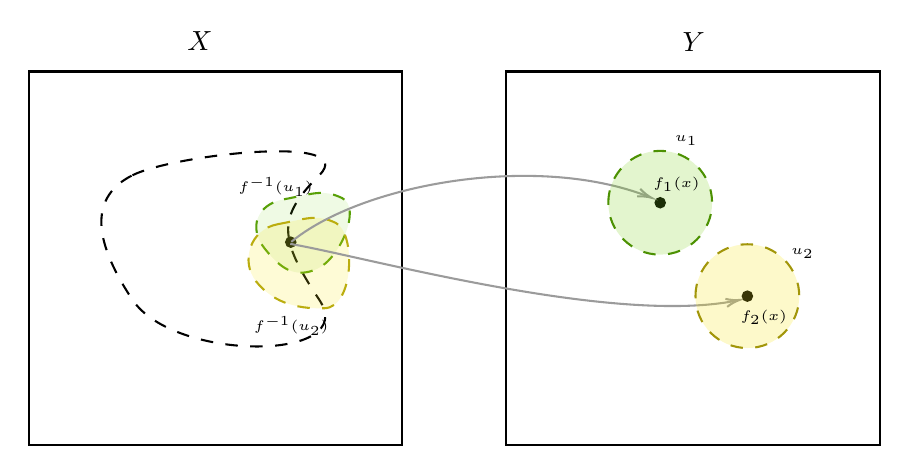
\begin{tikzpicture}[x=0.75pt,y=0.75pt,yscale=-1,xscale=1]
		%uncomment if require: \path (0,300); %set diagram left start at 0, and has height of 300
		
		%Shape: Circle [id:dp22945492936875378] 
		\draw  [fill={rgb, 255:red, 0; green, 0; blue, 0 }  ,fill opacity=1 ] (352,103.25) .. controls (352,102.01) and (353.01,101) .. (354.25,101) .. controls (355.49,101) and (356.5,102.01) .. (356.5,103.25) .. controls (356.5,104.49) and (355.49,105.5) .. (354.25,105.5) .. controls (353.01,105.5) and (352,104.49) .. (352,103.25) -- cycle ;
		%Shape: Square [id:dp934029333497959] 
		\draw   (50,40) -- (230,40) -- (230,220) -- (50,220) -- cycle ;
		%Shape: Square [id:dp16895777662650313] 
		\draw   (280,40) -- (460,40) -- (460,220) -- (280,220) -- cycle ;
		%Shape: Polygon Curved [id:ds9787457593928202] 
		\draw  [dash pattern={on 4.5pt off 4.5pt}] (100,90) .. controls (120,80) and (210,70) .. (190,90) .. controls (170,110) and (170,120) .. (190,150) .. controls (210,180) and (120,180) .. (100,150) .. controls (80,120) and (80,100) .. (100,90) -- cycle ;
		%Shape: Circle [id:dp057154404925263025] 
		\draw  [fill={rgb, 255:red, 0; green, 0; blue, 0 }  ,fill opacity=1 ] (174,122.25) .. controls (174,121.01) and (175.01,120) .. (176.25,120) .. controls (177.49,120) and (178.5,121.01) .. (178.5,122.25) .. controls (178.5,123.49) and (177.49,124.5) .. (176.25,124.5) .. controls (175.01,124.5) and (174,123.49) .. (174,122.25) -- cycle ;
		%Shape: Polygon Curved [id:ds5815057190055555] 
		\draw  [color={rgb, 255:red, 88; green, 160; blue, 7 }  ,draw opacity=1 ][fill={rgb, 255:red, 126; green, 211; blue, 33 }  ,fill opacity=0.12 ][dash pattern={on 4.5pt off 4.5pt}] (173,101.58) .. controls (186.5,99.08) and (191.5,96.42) .. (201,101) .. controls (210.5,105.58) and (200,130.08) .. (189,135.08) .. controls (178,140.08) and (171,134.58) .. (163.5,125.08) .. controls (156,115.58) and (159.5,104.08) .. (173,101.58) -- cycle ;
		%Shape: Polygon Curved [id:ds30989547801826567] 
		\draw  [color={rgb, 255:red, 187; green, 173; blue, 15 }  ,draw opacity=1 ][fill={rgb, 255:red, 248; green, 231; blue, 28 }  ,fill opacity=0.18 ][dash pattern={on 4.5pt off 4.5pt}] (170,113.58) .. controls (183.5,111.08) and (188.5,108.42) .. (198,113) .. controls (207.5,117.58) and (207,153.58) .. (192.5,154.08) .. controls (178,154.58) and (167,150.58) .. (159.5,141.08) .. controls (152,131.58) and (156.5,116.08) .. (170,113.58) -- cycle ;
		%Curve Lines [id:da29321026202366296] 
		\draw [color={rgb, 255:red, 155; green, 155; blue, 155 }  ,draw opacity=1 ][line width=0.75]    (176.5,122.08) .. controls (210.41,94.22) and (293.92,79.11) .. (348.36,100.19) ;
		\draw [shift={(350,100.84)}, rotate = 202.06] [color={rgb, 255:red, 155; green, 155; blue, 155 }  ,draw opacity=1 ][line width=0.75]    (6.56,-1.97) .. controls (4.17,-0.84) and (1.99,-0.18) .. (0,0) .. controls (1.99,0.18) and (4.17,0.84) .. (6.56,1.97)   ;
		%Curve Lines [id:da39067447551600165] 
		\draw [color={rgb, 255:red, 155; green, 155; blue, 155 }  ,draw opacity=1 ][line width=0.75]    (176,123.08) .. controls (211.15,129.02) and (330.58,162.4) .. (390.7,150.45) ;
		\draw [shift={(392.5,150.08)}, rotate = 167.68] [color={rgb, 255:red, 155; green, 155; blue, 155 }  ,draw opacity=1 ][line width=0.75]    (6.56,-1.97) .. controls (4.17,-0.84) and (1.99,-0.18) .. (0,0) .. controls (1.99,0.18) and (4.17,0.84) .. (6.56,1.97)   ;
		%Shape: Circle [id:dp16543584587564597] 
		\draw  [fill={rgb, 255:red, 0; green, 0; blue, 0 }  ,fill opacity=1 ] (394,148.25) .. controls (394,147.01) and (395.01,146) .. (396.25,146) .. controls (397.49,146) and (398.5,147.01) .. (398.5,148.25) .. controls (398.5,149.49) and (397.49,150.5) .. (396.25,150.5) .. controls (395.01,150.5) and (394,149.49) .. (394,148.25) -- cycle ;
		%Shape: Circle [id:dp376925694074147] 
		\draw  [color={rgb, 255:red, 76; green, 145; blue, 2 }  ,draw opacity=1 ][fill={rgb, 255:red, 126; green, 211; blue, 33 }  ,fill opacity=0.22 ][dash pattern={on 4.5pt off 4.5pt}] (329.25,103.25) .. controls (329.25,89.44) and (340.44,78.25) .. (354.25,78.25) .. controls (368.06,78.25) and (379.25,89.44) .. (379.25,103.25) .. controls (379.25,117.06) and (368.06,128.25) .. (354.25,128.25) .. controls (340.44,128.25) and (329.25,117.06) .. (329.25,103.25) -- cycle ;
		%Shape: Circle [id:dp3499499601701357] 
		\draw  [color={rgb, 255:red, 162; green, 150; blue, 10 }  ,draw opacity=1 ][fill={rgb, 255:red, 248; green, 231; blue, 28 }  ,fill opacity=0.23 ][dash pattern={on 4.5pt off 4.5pt}] (371.25,148.25) .. controls (371.25,134.44) and (382.44,123.25) .. (396.25,123.25) .. controls (410.06,123.25) and (421.25,134.44) .. (421.25,148.25) .. controls (421.25,162.06) and (410.06,173.25) .. (396.25,173.25) .. controls (382.44,173.25) and (371.25,162.06) .. (371.25,148.25) -- cycle ;
		
		% Text Node
		\draw (125,19.4) node [anchor=north west][inner sep=0.75pt]    {$X$};
		% Text Node
		\draw (363.5,19.9) node [anchor=north west][inner sep=0.75pt]    {$Y$};
		% Text Node
		\draw (349.5,89.4) node [anchor=north west][inner sep=0.75pt]  [font=\tiny]  {$f_{1}( x)$};
		% Text Node
		\draw (391.5,153.4) node [anchor=north west][inner sep=0.75pt]  [font=\tiny]  {$f_{2}( x)$};
		% Text Node
		\draw (360,69.4) node [anchor=north west][inner sep=0.75pt]  [font=\tiny]  {$u_{1}$};
		% Text Node
		\draw (416,123.9) node [anchor=north west][inner sep=0.75pt]  [font=\tiny]  {$u_{2}$};
		% Text Node
		\draw (149.5,89.4) node [anchor=north west][inner sep=0.75pt]  [font=\tiny]  {$f^{-1}( u_{1})$};
		% Text Node
		\draw (157,156.4) node [anchor=north west][inner sep=0.75pt]  [font=\tiny]  {$f^{-1}( u_{2})$};
		
		
	\end{tikzpicture}
\end{figure}
	
	\FloatBarrier
\end{proof}

\begin{remark}
	The theorem above indicates that if two continouse function from $\R \to \R$, agree on all values of the form $m/2^n$, for all $m\in\Z$ and $n\in \Z$, then they should agree on the whole real line.
\end{remark}

\section{Continuity and Compactness}
The compactness of the domain of a continouse function has many interesting implications.

\begin{theorem}[Continouse image of a compact set]
	Let $f:X\to Y$ be a continouse function, and $X$ compact. Then $f(X)$ is compact in $Y$.
\end{theorem}
\begin{proof}
	Let $\mathcal{G} = \{G_\alpha\}_{\alpha\in I}$ be an open cover for $f(X)$. Then we claim that $\tilde{\mathcal{G}} = \{ \inv{f}(G_\alpha) \}_{\alpha \in I}$ is also an open cover for $X$. That is because
	\[ \forall x \in X,\ \exists \alpha \in I \st f(x) \in G_\alpha \implies x \in \inv{f}(G_\alpha),\]
	thus the $\tilde{\mathcal{G}}$ covers every element of the set $X$. Since $X$ is compact, then there exists a finite sub-cover. I.e. there exists $I' \subseteq I$ finite such that $\tilde{\mathcal{G}}' = \{  \inv{f}(G_\alpha)  \}_{\alpha \in I'}$ is a finite cover for $X$. Now we claim that $\mathcal{G}' = \{  G_\alpha \}_{\alpha \in I'}$ is also a finite sub-cover for $f(X)$. This is true since for every $y \in f(X)$ we have
	\[ \inv{f}(y) \in X \implies \exists \alpha \in I' \st \inv{f}(y) \in \inv{f}(G_\alpha) \implies y \in G_\alpha. \]
	Thus $\mathcal{G}'$ covers every element of the set $f(X)$, thus it is a valid finite sub-cover for $\mathcal{G}$. This completes the proof.
\end{proof}